\newpage
\section{Ammonia Adsorption/Desorption Process Dynamics}

\begin{figure}[H]
    \centering
    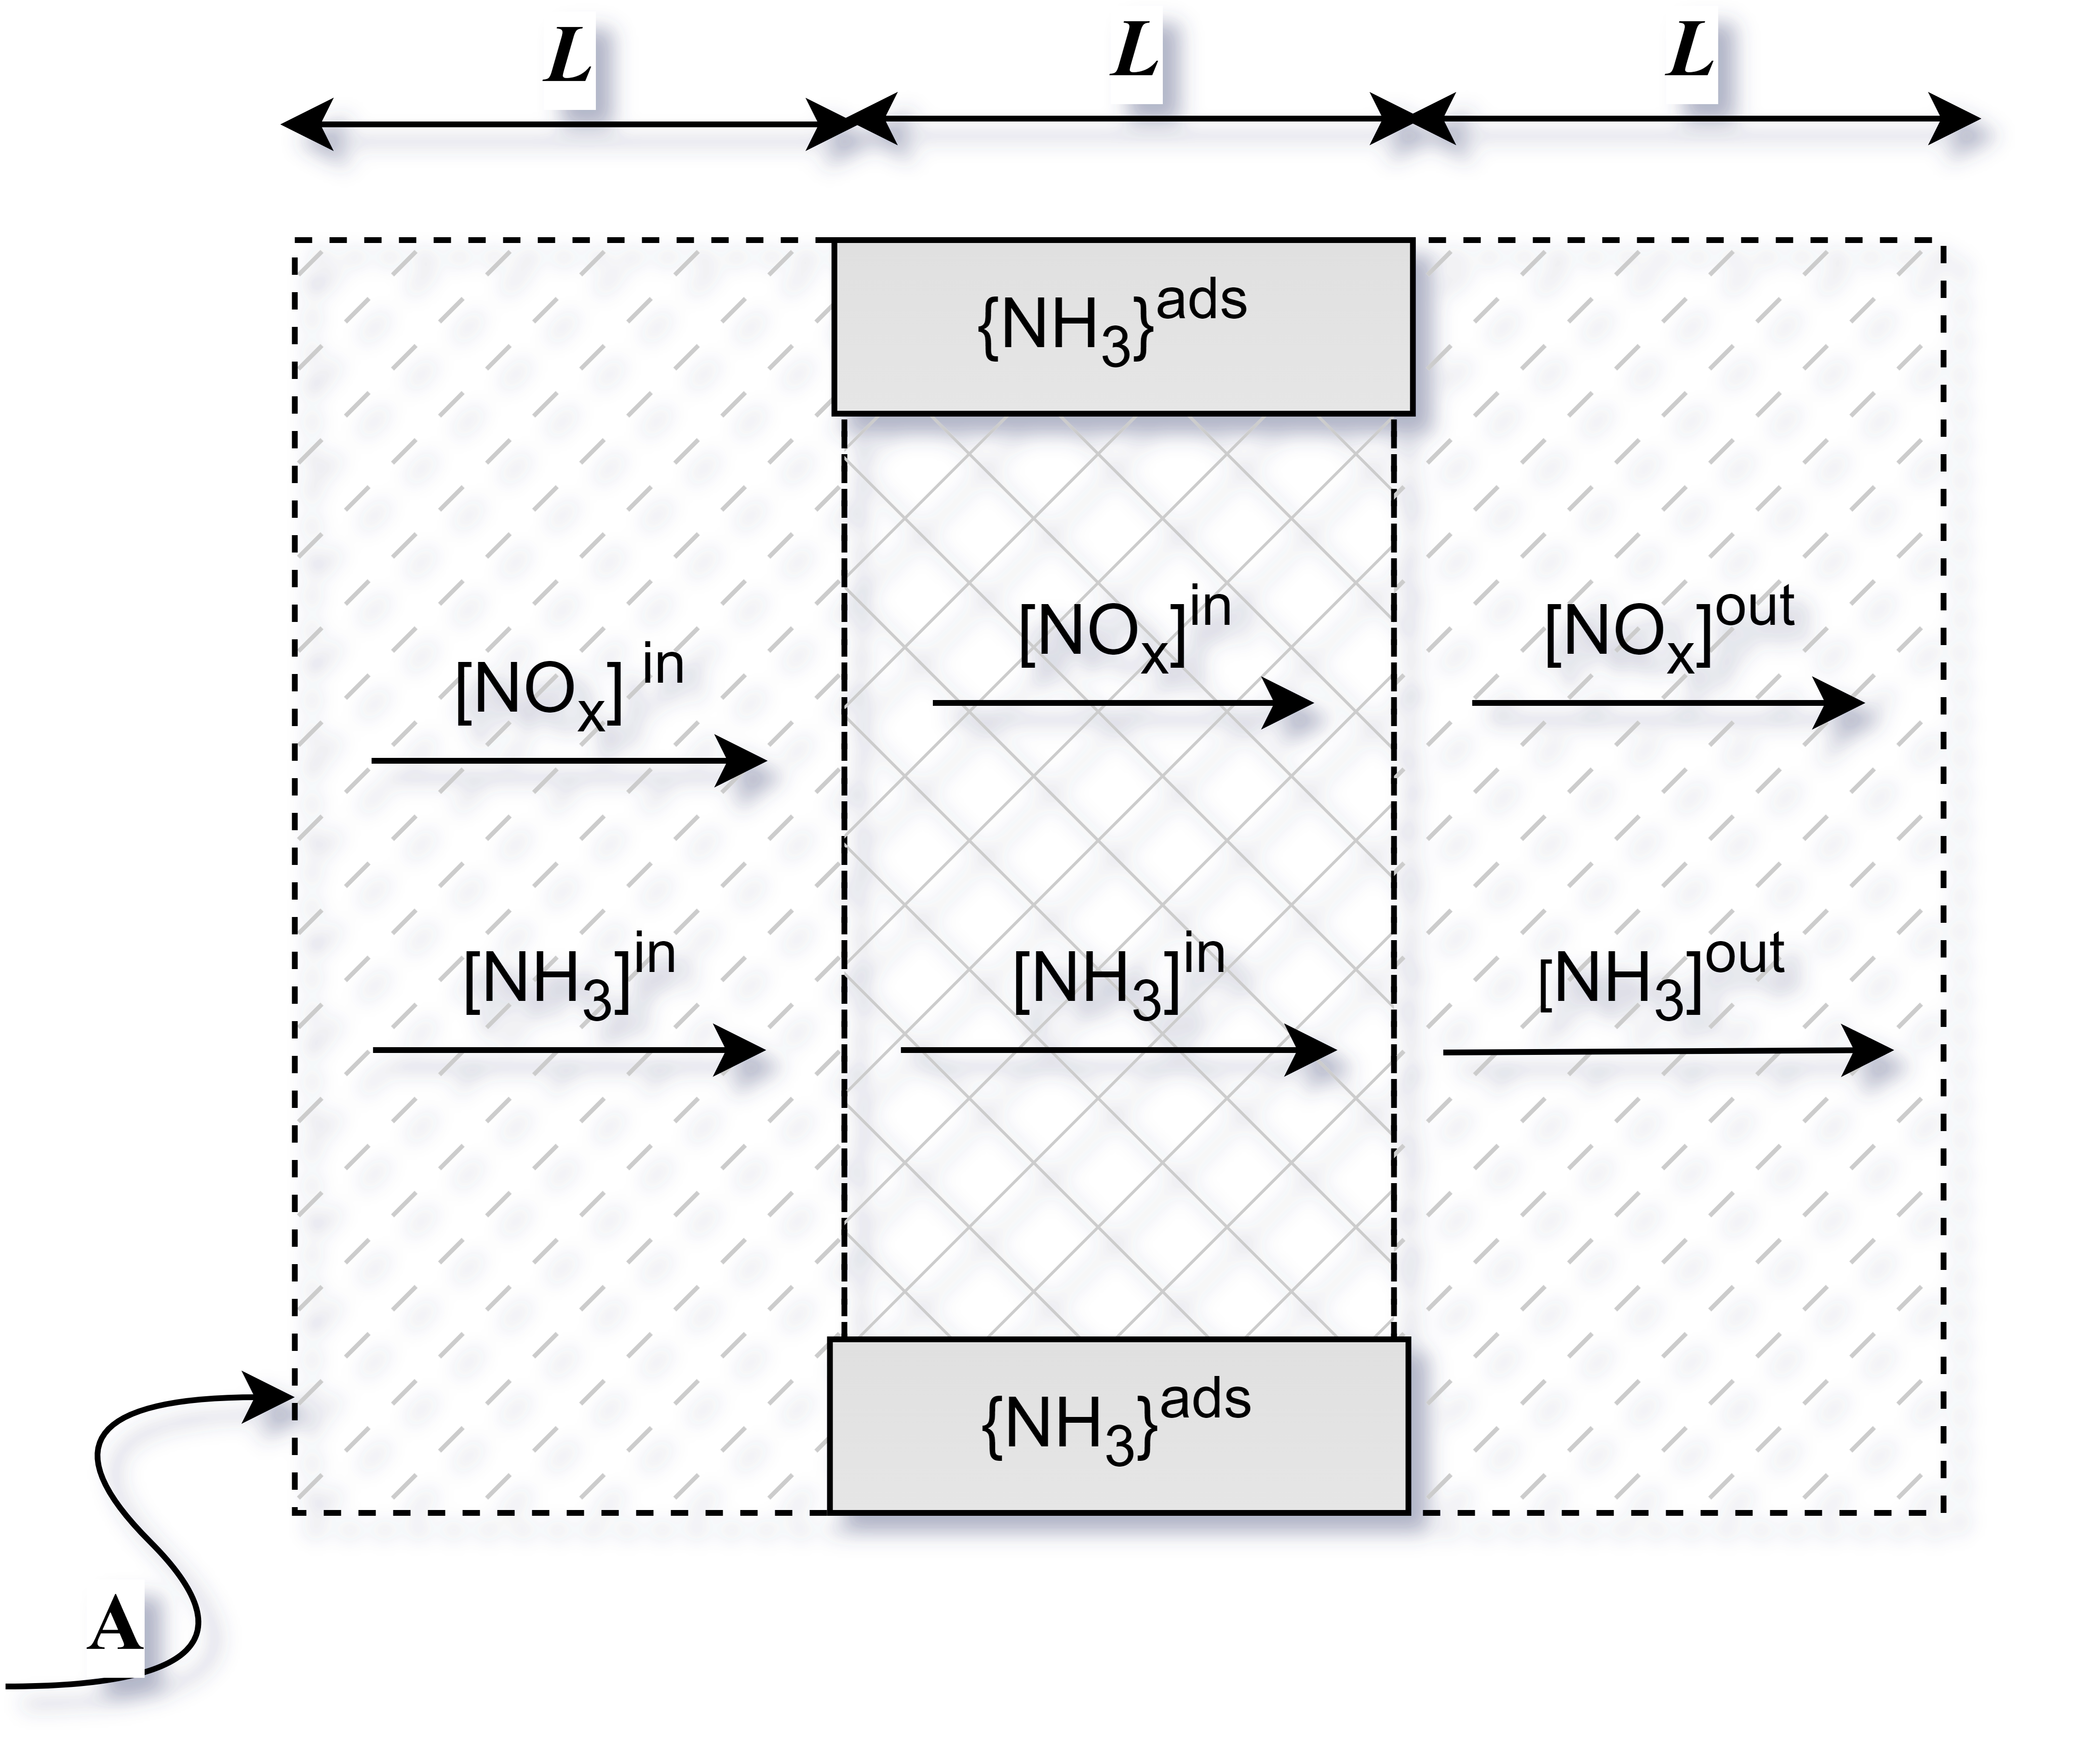
\includegraphics[width=0.5\textwidth]{./figs/scr_sys/plug_flow_discrete.png}
    \caption{Discrete plug-flow reactor model}
    \label{fig:plug_flow_discrete}
\end{figure}


The ammonia adsorption/desorption process dynamics involve all the three
above-mentioned reactions. The gaseous ammonia that enters the catalyst chamber
gets adsorbed on the to free sites on the catalyst surface at a rate
promotional to the volumetric concentration of the gaseous ammonia and the
surface concentration of the free sites. The adsorbed ammonia then either reacts
with the gaseous $NO_x$ (Eiley-Rideal Mechanism) releasing $N_2$ and $H_2O$ or
decomposes to form $N_2$ and $H_2O$ (Surface Decomposition). In either
case, the process frees up the adsorption sites for the next cycle of gasueous ammonia.

\begin{align*}
    4 NH_3 ^{ads} + 4 NO + O_2 &\xrightarrow[]{k_{scr}} 4 N_2 + 6 H_2O \\
    4 NH_3^{ads} + 3 O_2 &\xrightarrow[]{k_{oxi}} 2 N_2 + 6 H_2O \\
    NH_3 + \Theta_{free} &\xrightleftharpoons[k_{des}]{k_{ads}} NH_3^{ads}
\end{align*}


Thus, the rate of ammonia adsorption on the catalyst surface can be modeled as:

\begin{align*}
    \frac{d \con{NH_3}^{ads}}{dt} &= r_{ads} - r_{des} - r_{scr} - r_{oxi}\\
    r_{ads} &= k_{ads} \con{NH_3}^{in} \lr{\Gamma - \con{NH_3}^{ads}}\\
    r_{des} &= k_{des} \con{NH_3}^{ads}\\
    r_{scr} &= k_{scr} \con{NH_3}^{ads} \con{NO_x}^{in}\\
    r_{oxi} &= k_{oxi} \con{NH_3}^{ads}\\
    \dot{\con{NH_3}}^{ads} &= \Gamma \underbrace{k_{ads} \con{NH_3}^{in}}_{\gamma_{ads}} - \con{NH_3}^{ads} \underbrace{\lr{k_{ads} \con{NH_3}^{in} + k_{des} + k_{scr} \con{NO_x}^{in} + k_{oxi}}}_{\gamma_{des}}
\end{align*}

\itbf{Note:} $\Gamma$ and $\con{NH_3}^{ads}$ are surface concentrations (in
$moles/cm^2$) while the rest are volumetric concentrations (in $moles/cm^3$).
The rate constant units are adjusted appropriately to make the rate equations consistent.

The units of all the rates and rate constants are tabulated bellow:

\begin{align*}
    r_{ads} &= \frac{moles}{cm^2 \cdot s} &
    k_{ads} &= \frac{cm^3}{moles \cdot s} \\
    r_{des} &= \frac{moles}{cm^2 \cdot s} &
    k_{des} &= s^{-1} \\
    r_{scr} &= \frac{moles}{cm^2 \cdot s} &
    k_{scr} &= \frac{cm^3}{moles \cdot s} \\
    r_{oxi} &= \frac{moles}{cm^2 \cdot s} &
    k_{oxi} &= s^{-1}
\end{align*}


\itbf{Note:}In this section we are interested in the Surface rates where the
products are assumed to linger just on the surface of the catalyst. The surface
rates of the gaseous products/reactants are can be converted to volumetric
rates by using the convention factor $A_{scr}/V$ where $A_{scr}$ is the area of
the SCR catalyst and V is the volume of the catalyst chamber. This assumes that
there is instantaneous mixing of the close to  surface moles with the gaseous
moles. Thus,
\begin{align}
    k^{vol} = \underbrace{\lr{\frac{A_{scr}}{V}}}_{k_{s2v} \, (cm^{-1})} k^{surf}
\end{align}

% ==============================================================================

\subsection{Molar conservation at the scale of residence time}

The molar storage on the catalyst surface changes at the end of every residence
time and a "fresh" set of gaseous reactants enters the catalyst chamber. And,
with in the sample time, the volumetric concentrations of the gaseous reactants
can be considered constant. \itbf{Let there be $n$ residence times within one
sample time.} Then, the molar conservation for the adsorption/desorption process
can be written as:

\begin{align*}
    \mol{NH_3}^{ads} (k + \tau) &= \mol{NH_3}^{ads} (k) + A_{scr} \int_{0}^{\tau} \dot{\con{NH_3}}^{ads} (k) dt\\
    \mol{NH_3}^{ads} (k + 2\tau) &= \mol{NH_3}^{ads} (k + \tau) + A_{scr} \int_{0}^{\tau} \dot{\con{NH_3}}^{ads} (k + \tau) dt\\
    \vdots&\\
    \mol{NH_3}^{ads} (k + n\tau) &= \mol{NH_3}^{ads} (k + (n-1)\tau) + A_{scr} \int_{0}^{\tau} \dot{\con{NH_3}}^{ads} (k + (n-1)\tau) dt
\end{align*}

\begin{align*}
    \mol{NH_3}^{ads}(k + 1) = \mol{NH_3}^{ads} (k + n\tau) &= \mol{NH_3}^{ads} (k) + A_{scr} \sum_{i=0}^{n-1} \int_{0}^{\tau} \dot{\con{NH_3}}^{ads} (k + i\tau) dt
\end{align*}

Writing above equation interns of surface concentrations:
\begin{align*}
    \con{NH_3}^{ads}(k + 1) = \con{NH_3}^{ads} (k + n\tau) &= \con{NH_3}^{ads} (k) + \underbrace{\sum_{i=0}^{n-1} \int_{0}^{\tau} \dot{\con{NH_3}}^{ads} (k + i\tau)}_{\Omega(k)}   dt
\end{align*}

$\Omega(k)$ is the total change in the surface concentration of adsorbed ammonia
within one sample time.

% ==============================================================================
\subsection{Calculating the surface concentration change within one sample time $\Omega(k)$}

The volumetric concentrations of the gaseous reactants are assumed to be
constant within the sample time, while the surface concentrations change at the
end of every residence time.

\begin{align*}
    \dot{\con{NH_3}}^{ads} (k + i\tau) &= r_{ads} (k + i \tau) - r_{des} (k + i \tau) - r_{scr} (k + i \tau) - r_{oxi} (k + i \tau)\\
    %===
    r_{ads} (k + i \tau) &= k_{ads} \con{NH_3}^{in}(k) \lr{\Gamma - \con{NH_3}^{ads} (k + i \tau)}\\
    r_{des} (k + i \tau) &= k_{des} \con{NH_3}^{ads}(k + i \tau)\\
    r_{scr} (k + i \tau) &= k_{scr} \con{NH_3}^{ads}(k + i \tau) \con{NO_x}^{in}(k)\\
    r_{oxi} (k + i \tau) &= k_{oxi} \con{NH_3}^{ads}(k + i \tau)\\
    \gamma_{ads} (k) &= \Gamma k_{ads} \con{NH_3}^{in}(k)\\
    \gamma_{des} (k) &= \lr{k_{ads} \con{NH_3}^{in}(k) + k_{des} + k_{scr} \con{NO_x}^{in}(k) + k_{oxi}}\\
    %===
    \dot{\con{NH_3}}^{ads} (k + i\tau) &= \gamma_{ads} (k) - \con{NH_3}^{ads} (k + i \tau) \gamma_{des} (k)
\end{align*}

Calculating the expression for $\Omega(k)$:
\begin{align*}
    \Omega(k) &= \sum_{i=0}^{n-1} \int_{0}^{\tau} \dot{\con{NH_3}}^{ads} (k + i\tau) dt\\
    &= \sum_{i=0}^{n-1} \dot{\con{NH_3}}^{ads} (k + i\tau) \tau \qquad \lrb{\because \text{The rate is assumed to be constant within the residence time}}\\
    &= \sum_{i=0}^{n-1} \lr{\gamma_{ads} (k) - \con{NH_3}^{ads} (k + i \tau) \gamma_{des} (k)} \tau\\
    &= \tau n \Gamma \gamma_{ads} (k) - \tau \gamma_{des} (k) \underbrace{\sum_{i=0}^{n-1} \con{NH_3}^{ads} (k + i \tau) }_{n \sigma(k)} \\
    &= n \tau \lr{\Gamma \gamma_{ads} (k) - \sigma(k) \gamma_{des} (k)}
\end{align*}

The term $\sigma(k)$ is unknown and unobservable. It is the average surface
concentration at the end of every residence time within the sample time.

Moreover, we can get the expression for average rate of change of the surface
concentrations within the sample time as:
\begin{align*}
    \dot{\con{NH_3}}^{ads} (k) &= \frac{\Omega(k)}{\tau n} = \Gamma \gamma_{ads} (k) - \sigma(k) \gamma_{des} (k)\\
    &= \Gamma k_{ads} \con{NH_3}^{in}(k) - \sigma(k) \lr{k_{ads} \con{NH_3}^{in}(k) + k_{des} + k_{scr} \con{NO_x}^{in}(k) + k_{oxi}}
\end{align*}

% ==============================================================================

\subsection{Ammonia adsorption/desorption process dynamics model}
Substituting the expression for $\Omega(k)$ in the equation for
$\con{NH_3}^{ads}(k + 1)$:

\begin{align*}
    \con{NH_3}^{ads}(k + 1) &= \con{NH_3}^{ads} (k) + n \tau \lr{\Gamma \gamma_{ads} (k) - \sigma(k) \gamma_{des} (k)}\\
    &= \con{NH_3}^{ads}(k) + n \tau \Gamma k_{ads} \con{NH_3}^{in}(k) - n \tau \sigma(k) \lr{k_{ads} \con{NH_3}^{in}(k) + k_{des} + k_{scr} \con{NO_x}^{in}(k) + k_{oxi}}
\end{align*}

\subsection{Approximation of $\sigma(k)$ as $NH_3^{ads}(k)$ (Zero-order hold)}
\itbf{Note:} $\sigma(k)$ can be approximated as the surface concentration at the beginning of the sample time.

The average surface concentration $\sigma(k)$ in the sample time is approximated
as the surface concentration at the beginning of the sample time. This
approximation will introduce an error in the model whose effects will be
analyzed in sequential sections.

Thus,
\begin{align}
    \Omega(k) &\approx n \tau \lr{\Gamma \gamma_{ads} (k) - \con{NH_3}^{ads}(k) \gamma_{des} (k)}
\end{align}

Thus, we have approximate ammonia adsorption/desorption process dynamics model as:

\begin{align*}
    \con{NH_3}^{ads}(k + 1) &= \con{NH_3}^{ads} (k) + n \tau \lr{\Gamma \gamma_{ads} (k) - \con{NH_3}^{ads}(k) \gamma_{des} (k)}\\
    &= n \tau \Gamma \gamma_{ads} (k) + \con{NH_3}^{ads} (k) \lr{1 - n \tau \gamma_{des} (k)}\\
    &= n \tau \Gamma k_{ads} \con{NH_3}^{in}(k)  + \con{NH_3}^{ads} (k) \lr{1 - n \tau \lr{k_{ads} \con{NH_3}^{in}(k) + k_{des} + k_{scr} \con{NO_x}^{in}(k) + k_{oxi}}}
\end{align*}


\begin{align}
    \con{NH_3}^{ads}(k + 1) &= n \tau \Gamma k_{ads} \con{NH_3}^{in}(k)  + \con{NH_3}^{ads} (k) \lr{1 - n \tau \lr{k_{ads} \con{NH_3}^{in}(k) + k_{des} + k_{scr} \con{NO_x}^{in}(k) + k_{oxi}}}
\end{align}

Examining the individual terms:
\begin{align*}
    \con{NH_3}^{ads}(k + 1) =& \con{NH_3}^{ads}(k)\\
        &+ n\tau k_{ads} \con{NH_3}^{in} \lr{\Gamma - \con{NH_3}^{ads}(k)} \\
        &- n \tau \lr{k_{oxi} + k_{des}} \con{NH_3}^{ads} (k)\\
        &- n \tau k_{scr} \con{NO_x}^{in}(k) \con{NH_3}^{ads}(k)
\end{align*}

The above equation is nothing but multiplying the rate equation with the
sampling interval to get the measurement update.

Similarly, if we flip the approximation, that is if,
\begin{align*}
    \con{NH_3}^{ads}(k) &\approx \sigma(k)
\end{align*}
then,

\begin{align*}
    \sigma(k + 1) =& \sigma(k)\\
        &+ n\tau k_{ads} \con{NH_3}^{in} \lr{\Gamma - \sigma(k)} \\
        &- n \tau \lr{k_{oxi} + k_{des}} \sigma(k)\\
        &- n \tau k_{scr} \con{NO_x}^{in}(k) \sigma(k)
\end{align*}

